\documentclass[12pt]{article}	

\usepackage[margin=1in]{geometry}
\usepackage{amsmath,amssymb,amsthm}
\usepackage{graphicx}
\usepackage{caption}
\usepackage{subcaption}
\usepackage{url}
\usepackage{mathrsfs}
\newtheorem{theorem}{Theorem}
\newtheorem{notation}{Notation}
\newtheorem{claim}{Claim}
\newtheorem{lemma}{Lemma}
\newtheorem{definition}{Definition}
\renewcommand{\qedsymbol}{$\blacksquare$}
\newtheorem*{remark}{Remark}

\begin{document}
	\quad \quad \quad \quad \quad \quad \quad \quad \quad \quad  \quad \quad \quad \quad \quad \quad \quad \quad \quad \quad  \quad \quad \quad \quad \quad \quad \quad \quad \quad \quad  Arun Suresh
	\begin{center}
		Homework 5
	\end{center} 
	{\rule{\linewidth}{0.1mm} }

1. The objective of the problem was to sample and then perform a wavelet transform to the given function $$\psi(t) = \frac{2}{\sqrt[4]{\pi}\sqrt{3a}}(1-\frac{t^2}{a^2})\exp(-\frac{t^2}{2a^2})$$. 
However, before presenting my plots and results, I would like to present the plots that I obtained from a different function - as a proof of concept that the wavelet transform being performed is performing as predicted. I performed this sample experiment because - the wavelet transform on the given $\psi$ function returned coefficients (at least low-pass ones) that didn't quite show any significant shape changes as I progressed down the layers (but there were significant scaling differences), and so I needed a high frequency sample function to absolutely make sure that my code was indeed working. As a sample function, I used the chirp function $$f(x) = \sin(250\pi x^2)$$ the plot of which is presented below. \\
\begin{figure}[h]
	\centering
	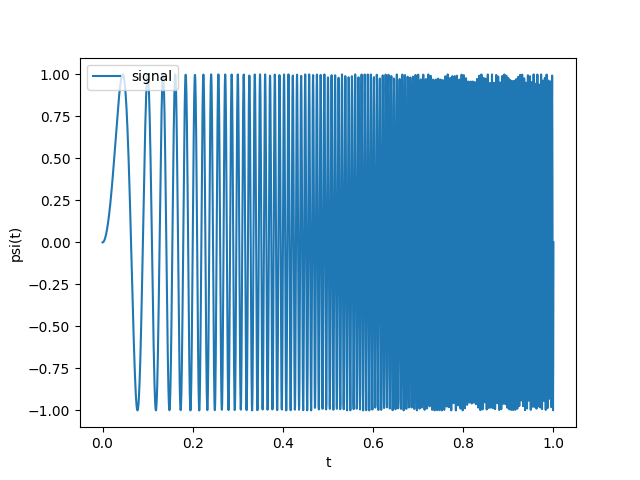
\includegraphics[scale=0.40]{proofofconcept.png}
	\caption{Chirp function}
\end{figure}\\\\
For this, we chose the DAUB5 mother wavelet to perform a wavelet transformation. To this function, I performed a discrete wavelet transformation, and then to the result, performed an inverse wavelet transformation provided by the PyWavelets package in python. The transform was performed over five pass-filters, and coefficients from each pass-filter was recorded in the process. The plots of the reconstructed chirp function, along with coefficients from each of the layers are presented below. 
\begin{figure}[h]
	\centering
	\begin{subfigure}[h]{0.40\textwidth}
		\centering
		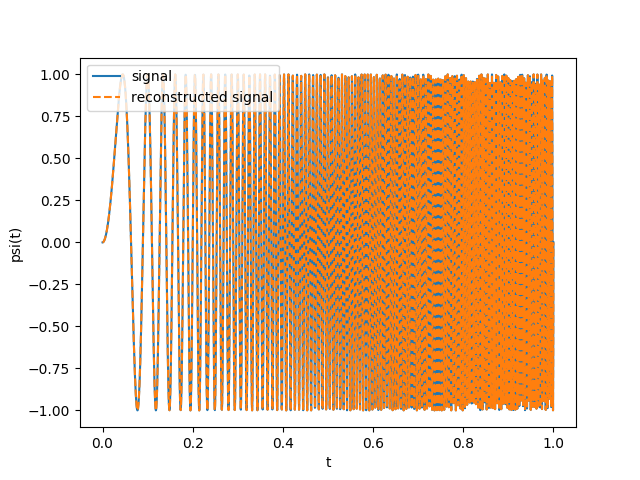
\includegraphics[width=\textwidth]{proofofconcept_reconst.png}
		\caption{Reconstructed signal}
	\end{subfigure}
	\begin{subfigure}[h]{0.40\textwidth}
		\centering
		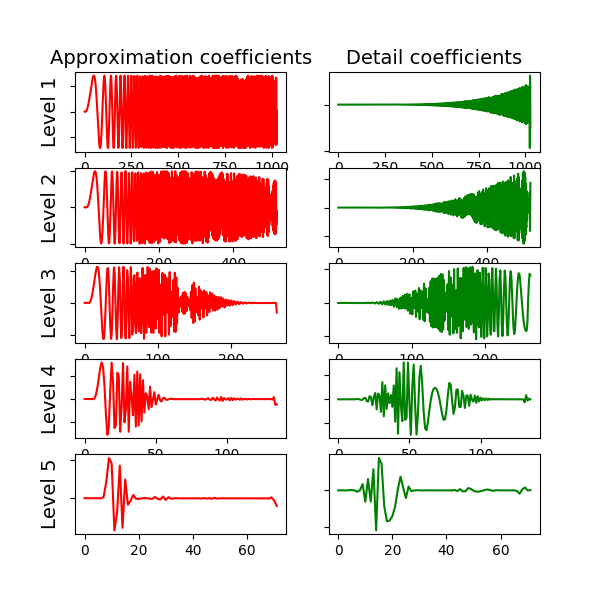
\includegraphics[width=\textwidth]{proofofconcept_coeff.png}
		\caption{Coefficients from different levels}
	\end{subfigure}
	\caption{Wavelet transforms of Chirp function}
\end{figure}
\\\\
\indent \newpage It is clear that the reconstructed signal approximates the actual signal to a very good extent. Figure(2), plot (b) contains information about the high pass and low pass coefficients of the transform. The plots in red correspond to coefficients from the low pass filter (lower-end approximation), and the plots in green correspond to coefficients from high pass filter (high-end approximation), at each level. Just as expected, we see that the amount of detail we need reduces as the levels go deeper and deeper - as the frequency range for analysis gets lower and lower (at level five, we are working $\frac{1}{16}^{th}$ of the maximum frequency). \\
\indent Now that we have gotten past this proof of concept - we can finally analyze the reconstruction and coefficient plots of the given $\psi(t)$. Presented below are the corresponding plots when the mother wavelet was the Haar wavelet.  
\begin{figure}[h]
	\centering
	\begin{subfigure}[h]{0.40\textwidth}
		\centering
		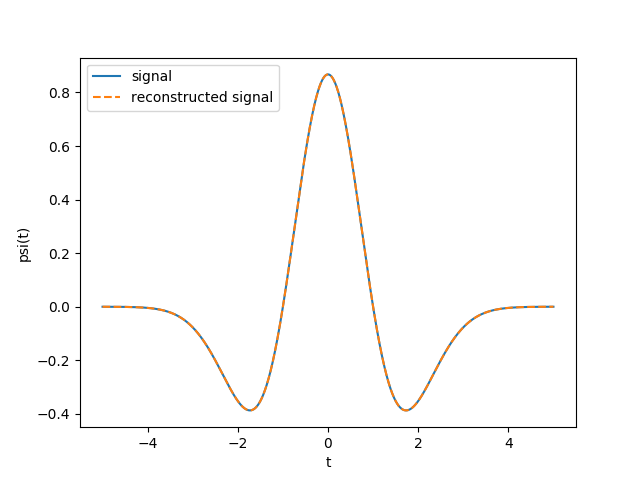
\includegraphics[width=\textwidth]{wavelet_reconst_haar.png}
		\caption{Reconstructed signal}
	\end{subfigure}
	\begin{subfigure}[h]{0.40\textwidth}
		\centering
		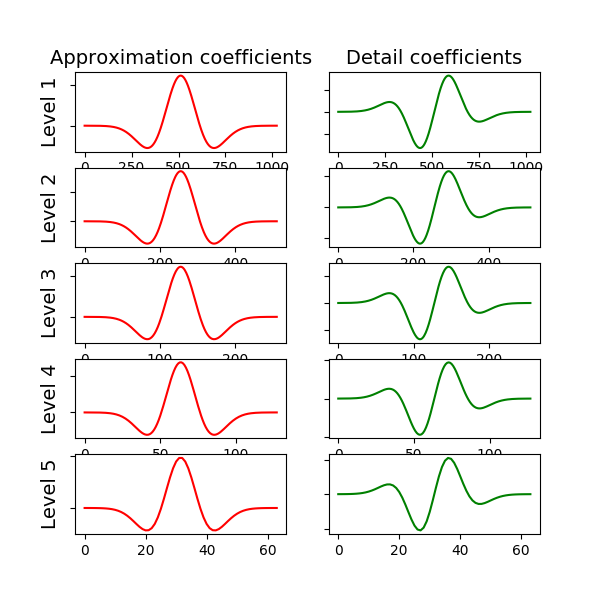
\includegraphics[width=\textwidth]{Wavelet_coeff_Haar.png}
		\caption{Coefficients from different levels}
	\end{subfigure}
	\caption{Haar - wavelet transforms of $\psi(x)$}
\end{figure}\\\\ 
In addition, presented below is reconstruction and coefficient plots $\psi(t)$ when the mother function was DAUB5
\begin{figure}[h]
	\centering
	\begin{subfigure}[h]{0.40\textwidth}
		\centering
		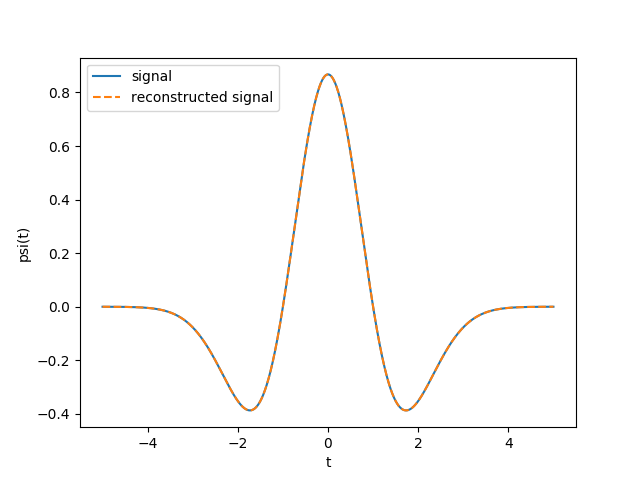
\includegraphics[width=\textwidth]{wavelet_reconst_db5.png}
		\caption{Reconstructed signal}
	\end{subfigure}
	\begin{subfigure}[h]{0.40\textwidth}
		\centering
		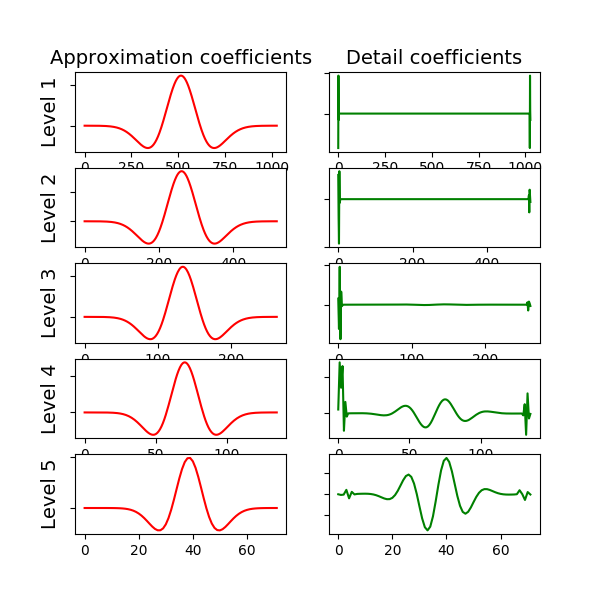
\includegraphics[width=\textwidth]{Wavelet_coeff_db5.png}
		\caption{Coefficients from different levels}
	\end{subfigure}
	\caption{DAUB5 - wavelet transforms of $\psi(x)$}
\end{figure}

Notice that the reconstruction is very accurate in the case of both mother wavelets, but there are huge differences in the high-pass coefficients. This is very much expected out of the differences between the Haar wavelet and DAUB 5 wavelets that are reproduced below. 

\begin{figure}[h]
	\centering
	\begin{subfigure}[h]{0.20\textwidth}
		\centering
		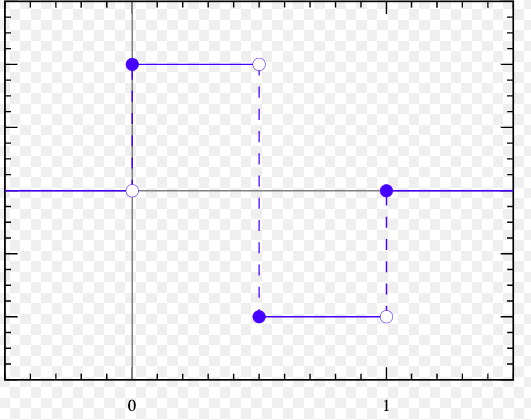
\includegraphics[width=\textwidth]{haar.png}
		\caption{Haar function}
	\end{subfigure}
	\begin{subfigure}[h]{0.20\textwidth}
		\centering
		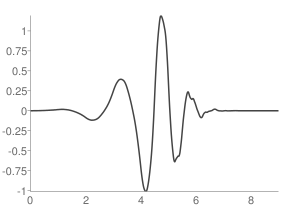
\includegraphics[width=\textwidth]{daub5.png}
		\caption{Daubechies 5}
	\end{subfigure}
	\caption{DAUB5 - wavelet transforms of $\psi(x)$}
\end{figure}

It is expected that the lower end approximations of a very simple wavelet like function such as $\psi(t)$ are more or less the same shape in every level and merely require re-scaling, but higher level smoothing coefficients are forced to be considerably different. Notice also that, the haar function (which has abdrupt discontinuity) coefficients needed a significant amount of higher order smoothing across the domain, whereas in the Daub5 (comparitively more continuous) we do not require a lot of higher order smoothing, and only need them to reduce the edge effects. And we also notice the dominance of low-frequency wavelets in the central area of the function (which is very expected) and higher order frequencies with high pass filters, are filtered out in the initial layers.


\end{document}